% Diagrama de flujo del firmware del nodo ESP32 (reglas F1-F7 de docs/guia-diagramas.md).
% Dos columnas unidas por conectores circulares (simbologia estandar ANSI/ISO 5807):
%   columna izquierda = inicializacion, adquisicion y seguridad CO;
%   columna derecha   = conectividad MQTT, control y publicacion.
%   A: continua en "¿MQTT conectado?"; B: retorno al inicio del bucle.
% F1 simbologia: ovalo inicio, rectangulo proceso, rombo decision, paralelogramo E/S, circulo conector.
% F5: CO es la primera decision de control; antes solo se comprueba que haya lectura nueva y que los
%     MQ hayan terminado el precalentamiento (sin eso la lectura de CO no es valida -> co_valid=0).
%     La alarma se enclava y solo se libera con CO < 50 - h ppm. Durante la alarma la telemetria sigue.
% F6: temporizadores millis(), sin delay(): muestreo T_s, telemetria T, precalentamiento t_warm,
%     encendido minimo 60 s. La alarma se publica solo al cambiar (flanco), no en cada vuelta.
% Decision del orquestador (DIA-2-04): histeresis +-0.5 C y encendido minimo 60 s son del lazo local
%     del firmware; la heuristica del backend solo envia modo/consigna/fan_pwm por cmd.
% [CONFIRMAR] T_s, T, t_warm, h, histeresis y 60 s en el firmware (P-08); ventilador sin red.
% Alto natural <= 440 pt: incluir a tamano natural o width=\linewidth, nunca escalado por altura.
\documentclass[tikz,border=4pt]{standalone}
\usepackage[utf8]{inputenc}
\usepackage[T1]{fontenc}
\usepackage{lmodern}
\usetikzlibrary{shapes.geometric, arrows.meta, positioning, fit, backgrounds, calc}

\definecolor{acento}{RGB}{176,30,30}   % unico acento: rama de seguridad CO

\tikzset{
  base/.style      = {draw, thick, align=center, font=\fontsize{7.5}{8.6}\selectfont, inner sep=2pt},
  startstop/.style = {base, ellipse, fill=gray!25, minimum width=18mm, minimum height=6.5mm},
  process/.style   = {base, rectangle, fill=gray!10, minimum height=7mm},
  io/.style        = {base, trapezium, trapezium left angle=72, trapezium right angle=108,
                      trapezium stretches body, fill=white, minimum height=7mm},
  decision/.style  = {base, diamond, aspect=2.5, fill=gray!18, inner sep=0.8pt},
  conector/.style  = {draw, thick, circle, fill=white, minimum size=4.2mm, inner sep=0pt,
                      font=\fontsize{7.5}{7.5}\selectfont\bfseries},
  seguridad/.style = {draw=acento, very thick},
  flow/.style      = {-{Stealth[length=1.8mm]}, thin},
  aflow/.style     = {flow, acento, thick},
  vf/.style        = {font=\fontsize{7.5}{7.5}\selectfont\bfseries, inner sep=1.5pt},
  nota/.style      = {font=\fontsize{7}{7.8}\selectfont\itshape, text=gray!30!black, align=left},
}

\begin{document}
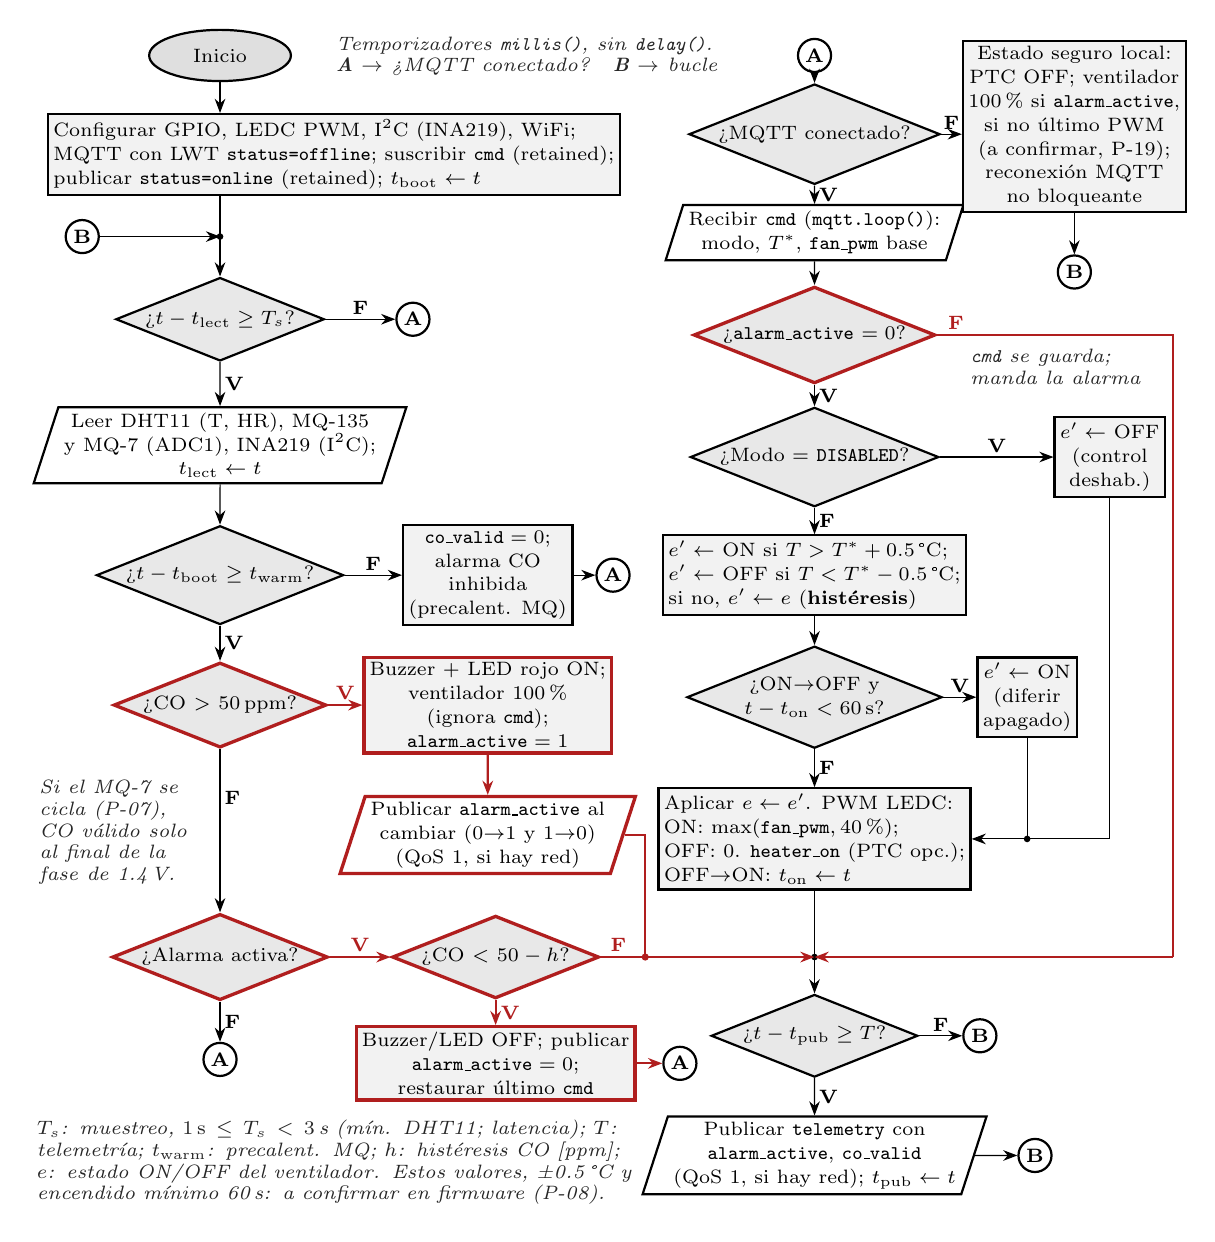
\begin{tikzpicture}

% =====================================================================
% Columna izquierda: inicializacion, adquisicion y seguridad CO (x = 0)
% =====================================================================
\node[startstop] (ini) at (0,0) {Inicio};
\node[process, anchor=north west, align=left] (cfg) at (-2.2,-0.73)
  {Configurar GPIO, LEDC PWM, I\textsuperscript{2}C (INA219), WiFi;\\
   MQTT con LWT \texttt{status=offline}; suscribir \texttt{cmd} (retained);\\
   publicar \texttt{status=online} (retained); $t_{\mathrm{boot}} \leftarrow t$};
\coordinate (L) at (0,-2.3);
\node[conector] (Bin) at (-1.75,-2.3) {B};
\node[decision] (ts)  at (0,-3.35) {¿$t - t_{\mathrm{lect}} \geq T_s$?};
\node[io]       (rd)  at (0,-4.95) {Leer DHT11 (T, HR), MQ-135\\y MQ-7 (ADC1), INA219 (I\textsuperscript{2}C);\\$t_{\mathrm{lect}} \leftarrow t$};
\node[decision] (wm)  at (0,-6.6)  {¿$t - t_{\mathrm{boot}} \geq t_{\mathrm{warm}}$?};
\node[decision, seguridad] (co) at (0,-8.25) {¿CO $>$ 50\,ppm?};
\node[decision, seguridad] (aa) at (0,-11.45) {¿Alarma activa?};
\node[conector] (A3) at (0,-12.75) {A};

\draw[flow] (ini) -- (ini |- cfg.north);
\draw (ini |- cfg.south) -- (L);
\draw[flow] (Bin) -- (L);
\fill (L) circle (1.2pt);
\draw[flow] (L) -- (ts);
\draw[flow] (ts) -- node[vf, right] {V} (rd);
\draw[flow] (rd) -- (wm);
\draw[flow] (wm) -- node[vf, right] {V} (co);
\draw[flow] (co) -- node[vf, right, pos=0.3] {F} (aa);
\node[nota, anchor=north west, inner sep=0pt] at (-2.3,-9.2)
  {Si el MQ-7 se\\cicla (P-07),\\CO válido solo\\al final de la\\fase de 1.4\,V.};
\draw[flow] (aa) -- node[vf, right] {F} (A3);

% sin lectura nueva -> A
\node[conector] (A1) at (2.45,-3.35) {A};
\draw[flow] (ts) -- node[vf, above] {F} (A1);

% precalentamiento MQ: lectura de CO no valida, alarma inhibida
\node[process] (cov) at (3.4,-6.6) {\texttt{co\_valid}${}=0$;\\alarma CO\\inhibida\\(precalent. MQ)};
\draw[flow] (wm) -- node[vf, above] {F} (cov);

% ---------------- rama de seguridad CO (prioridad maxima) ----------------
\node[process, seguridad] (alarm) at (3.4,-8.25)
  {Buzzer + LED rojo ON;\\ventilador 100\,\%\\(ignora \texttt{cmd});\\\texttt{alarm\_active}${}=1$};
\node[io, seguridad] (palarm) at (3.4,-9.9) {Publicar \texttt{alarm\_active} al\\cambiar (0$\rightarrow$1 y 1$\rightarrow$0)\\(QoS 1, si hay red)};
\draw[aflow] (co) -- node[vf, above, text=acento] {V} (alarm);
\draw[aflow] (alarm) -- (palarm);

% salida de la alarma con histeresis
\node[decision, seguridad] (hy) at (3.5,-11.45) {¿CO $<$ $50-h$?};
\draw[aflow] (aa) -- node[vf, above, text=acento] {V} (hy);
\node[process, seguridad] (off) at (3.5,-12.8)
  {Buzzer/LED OFF; publicar\\\texttt{alarm\_active}${}=0$;\\restaurar último \texttt{cmd}};
\draw[aflow] (hy) -- node[vf, right, text=acento] {V} (off);
\node[conector] (A4) at ($(off.east)+(0.55,0)$) {A}; % DIA-5-02: caja off mas ancha
\draw[aflow] (off) -- (A4);

% alarma activa o enclavada -> M (la telemetria sigue saliendo durante el evento)
\coordinate (G) at (5.4,-11.45);
\draw[acento, thick] (palarm.east) -| (G);
\draw[acento, thick] (hy.east) -- node[vf, above, text=acento, pos=0.4] {F} (G);
\fill[acento] (G) circle (1.3pt);

% =====================================================================
% Columna derecha: conectividad, control y publicacion (x = 7.55)
% DIA-3-01: con alarm_active = 1 ningun camino llega al lazo local (rombo cmd, rama F -> M).
% DIA-4-01: lazo local con histeresis en ambos sentidos sobre el estado e del ventilador:
%   e' = ON si T > T*+0.5; OFF si T < T*-0.5; si no, e' = e. ON -> PWM = max(fan_pwm, 40 %); OFF -> 0.
%   Modo DISABLED (de cmd) -> e' = OFF siempre. Los 60 s son tiempo minimo de ENCENDIDO:
%   solo bloquean la transicion ON -> OFF (e' <- ON); no frenan el encendido ni el resto del lazo,
%   y un fan_pwm nuevo se aplica aunque el apagado este diferido.
% Carriles a la derecha: x = 10.25 (encendido minimo), 11.3 (DISABLED), 12.1 (alarma -> M). Sin cruces.
% =====================================================================
\def\xc{7.55}
\node[conector] (Ain) at (\xc,0) {A};
\node[decision] (mq)  at (\xc,-1.0) {¿MQTT conectado?};
\node[io] (lp) at (\xc,-2.25) {Recibir \texttt{cmd} (\texttt{mqtt.loop()}):\\modo, $T^{*}$, \texttt{fan\_pwm} base};
\node[decision, seguridad] (cmd) at (\xc,-3.55)  {¿\texttt{alarm\_active} $=0$?};
\node[decision] (dis) at (\xc,-5.1) {¿Modo $=$ \texttt{DISABLED}?};
\node[process, align=left] (hys) at (\xc,-6.6)
  {$e' \leftarrow$ ON si $T > T^{*}+0.5$\,°C;\\
   $e' \leftarrow$ OFF si $T < T^{*}-0.5$\,°C;\\
   si no, $e' \leftarrow e$ (\textbf{histéresis})};
\node[decision] (mn) at (\xc,-8.15) {¿ON$\rightarrow$OFF y\\$t - t_{\mathrm{on}} < 60$\,s?};
\node[process, align=left] (ap) at (\xc,-9.95)
  {Aplicar $e \leftarrow e'$. PWM LEDC:\\
   ON: $\max(\texttt{fan\_pwm}, 40\,\%)$;\\
   OFF: 0. \texttt{heater\_on} (PTC opc.);\\
   OFF$\rightarrow$ON: $t_{\mathrm{on}} \leftarrow t$};
% DIA-5-01: conector A de precalentamiento a >= 4 mm de hys.west (radio 2.1 mm + 4 mm)
\node[conector] (A2) at ($(hys.west)+(-0.62,0)$) {A};
\draw[flow] (cov) -- (A2);
\coordinate (M) at (\xc,-11.45);
\node[decision] (tp)  at (\xc,-12.45) {¿$t - t_{\mathrm{pub}} \geq T$?};
\node[io] (pub) at (\xc,-13.97) {Publicar \texttt{telemetry} con\\\texttt{alarm\_active}, \texttt{co\_valid}\\(QoS 1, si hay red); $t_{\mathrm{pub}} \leftarrow t$};
\node[conector] (B3) at (10.35,-13.97) {B};

\draw[flow] (Ain) -- (mq);
\draw[flow] (mq) -- node[vf, right] {V} (lp);
\draw[flow] (lp) -- (cmd);
\draw[flow] (cmd) -- node[vf, right] {V} (dis);
\draw[flow] (dis) -- node[vf, right] {F} (hys);
\draw[flow] (hys) -- (mn);
\draw[flow] (mn) -- node[vf, right] {F} (ap);
\draw (ap) -- (M);
\draw[flow] (M) -- (tp);
\draw[flow] (tp) -- node[vf, right] {V} (pub);
\draw[flow] (pub) -- (B3);
\fill (M) circle (1.2pt);

% DISABLED: ventilador OFF siempre (no pasa por histeresis ni por el encendido minimo)
\node[process] (doff) at (11.3,-5.1) {$e' \leftarrow$ OFF\\(control\\deshab.)};
\draw[flow] (dis) -- node[vf, above] {V} (doff);
% encendido minimo: solo bloquea la transicion ON -> OFF
\node[process] (keep) at (10.25,-8.15) {$e' \leftarrow$ ON\\(diferir\\apagado)};
\draw[flow] (mn) -- node[vf, above] {V} (keep);
\coordinate (J) at (11.3,-9.95);
\draw (doff) -- (J);
\draw (keep) -- (keep |- ap.east);
\draw[flow] (J) -- (ap.east);
\fill (keep |- ap.east) circle (1.2pt);

% rama de alarma entra a M desde la columna izquierda
\draw[aflow] (G) -- (M);

% sin red: estado seguro local -> B
\node[process, anchor=north] (safe) at (10.85,0.2)
  {Estado seguro local:\\PTC OFF; ventilador\\100\,\% si \texttt{alarm\_active},\\si no último PWM\\(a confirmar, P-19);\\reconexión MQTT\\no bloqueante};
\draw[flow] (mq) -- node[vf, above] {F} (mq -| safe.west);
\node[conector] (B1) at (10.85,-2.75) {B};
\draw[flow] (safe) -- (B1);

% alarma activa: cmd guardado, no se aplica -> M
\coordinate (R) at (12.1,-11.45);
\draw[acento, thick] (cmd.east) -- node[vf, above, text=acento, pos=0.08] {F} (cmd.east -| R) -- (R);
\draw[aflow] (R) -- (M);
\node[nota, anchor=north west] at ($(cmd.east)+(0.3,-0.06)$) {\texttt{cmd} se guarda;\\manda la alarma};

% sin telemetria pendiente -> B
\node[conector] (B2) at (9.65,-12.45) {B};
\draw[flow] (tp) -- node[vf, above] {F} (B2);

% ---------------- notas ----------------
% arriba (entre Inicio y la columna derecha): temporizadores y conectores
\node[nota, anchor=north west] at (1.35,0.36)
  {Temporizadores \texttt{millis()}, sin \texttt{delay()}.\\
   \textbf{A} $\rightarrow$ ¿MQTT conectado?\quad \textbf{B} $\rightarrow$ bucle};
% abajo a la izquierda: definiciones y valores a confirmar
\node[nota, anchor=north west, text width=77mm] at (-2.45,-13.4)
  {$T_s$: muestreo, $1\,\mathrm{s} \leq T_s < 3$\,s (mín. DHT11; latencia);
   $T$: telemetría; $t_{\mathrm{warm}}$: precalent. MQ; $h$: histéresis CO [ppm];
   $e$: estado ON/OFF del ventilador. Estos valores, ±0.5\,°C y encendido mínimo 60\,s:
   a confirmar en firmware (P-08).};

\end{tikzpicture}
\end{document}
